\subsection{Time dependent coordinate transformation}
wave equation

\subsection{orbital parameters (osculating orbits paper)}
\subsection{precession figure}
chi(t),psir,psirtheta,psirphi,psirt

\begin{figure}
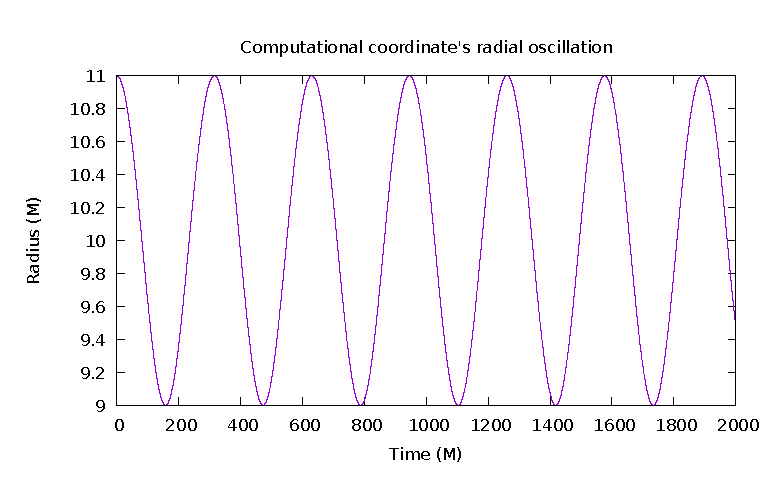
\includegraphics{/home/sdorsher/LabNotebook/20170713/orbit}
\end{figure}




\begin{figure}
  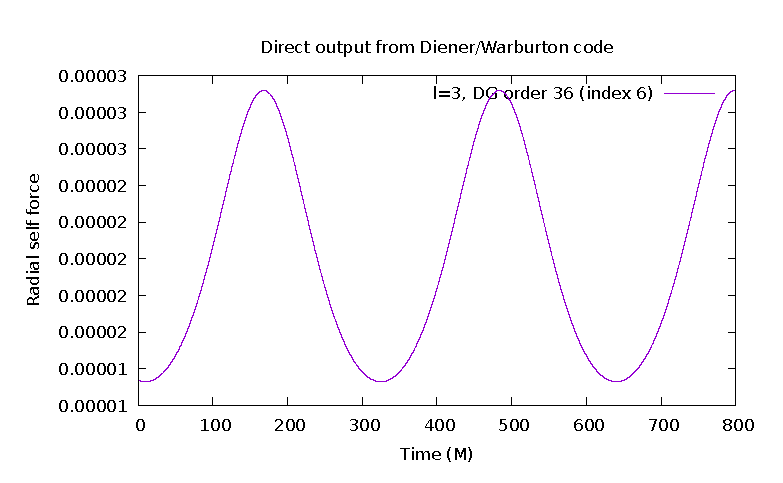
\includegraphics{/home/sdorsher/LabNotebook/20170714/psirl_l3_order36}
  \caption{470 M near perihelion, 640 M at aphelion}
\end{figure}
